\batchmode

\documentclass[letterpaper,12pt]{article}
\RequirePackage{ifthen}




\usepackage{pdflscape}
\usepackage{longtable}
\usepackage{url}
\usepackage{graphicx}
\usepackage{paralist}
\usepackage{comment}
\usepackage{color}
\usepackage[left=3cm,top=3cm,right=3cm, bottom=3cm,nohead]{geometry}
\usepackage{booktabs}


\title{Supplementary materials for Fish and Fisheries manuscript}





\pagecolor[gray]{.7}

\usepackage[]{inputenc}



\makeatletter

\makeatletter
\count@=\the\catcode`\_ \catcode`\_=8 
\newenvironment{tex2html_wrap}{}{}%
\catcode`\<=12\catcode`\_=\count@
\newcommand{\providedcommand}[1]{\expandafter\providecommand\csname #1\endcsname}%
\newcommand{\renewedcommand}[1]{\expandafter\providecommand\csname #1\endcsname{}%
  \expandafter\renewcommand\csname #1\endcsname}%
\newcommand{\newedenvironment}[1]{\newenvironment{#1}{}{}\renewenvironment{#1}}%
\let\newedcommand\renewedcommand
\let\renewedenvironment\newedenvironment
\makeatother
\let\mathon=$
\let\mathoff=$
\ifx\AtBeginDocument\undefined \newcommand{\AtBeginDocument}[1]{}\fi
\newbox\sizebox
\setlength{\hoffset}{0pt}\setlength{\voffset}{0pt}
\addtolength{\textheight}{\footskip}\setlength{\footskip}{0pt}
\addtolength{\textheight}{\topmargin}\setlength{\topmargin}{0pt}
\addtolength{\textheight}{\headheight}\setlength{\headheight}{0pt}
\addtolength{\textheight}{\headsep}\setlength{\headsep}{0pt}
\setlength{\textwidth}{349pt}
\newwrite\lthtmlwrite
\makeatletter
\let\realnormalsize=\normalsize
\global\topskip=2sp
\def\preveqno{}\let\real@float=\@float \let\realend@float=\end@float
\def\@float{\let\@savefreelist\@freelist\real@float}
\def\liih@math{\ifmmode$\else\bad@math\fi}
\def\end@float{\realend@float\global\let\@freelist\@savefreelist}
\let\real@dbflt=\@dbflt \let\end@dblfloat=\end@float
\let\@largefloatcheck=\relax
\let\if@boxedmulticols=\iftrue
\def\@dbflt{\let\@savefreelist\@freelist\real@dbflt}
\def\adjustnormalsize{\def\normalsize{\mathsurround=0pt \realnormalsize
 \parindent=0pt\abovedisplayskip=0pt\belowdisplayskip=0pt}%
 \def\phantompar{\csname par\endcsname}\normalsize}%
\def\lthtmltypeout#1{{\let\protect\string \immediate\write\lthtmlwrite{#1}}}%
\newcommand\lthtmlhboxmathA{\adjustnormalsize\setbox\sizebox=\hbox\bgroup\kern.05em }%
\newcommand\lthtmlhboxmathB{\adjustnormalsize\setbox\sizebox=\hbox to\hsize\bgroup\hfill }%
\newcommand\lthtmlvboxmathA{\adjustnormalsize\setbox\sizebox=\vbox\bgroup %
 \let\ifinner=\iffalse \let\)\liih@math }%
\newcommand\lthtmlboxmathZ{\@next\next\@currlist{}{\def\next{\voidb@x}}%
 \expandafter\box\next\egroup}%
\newcommand\lthtmlmathtype[1]{\gdef\lthtmlmathenv{#1}}%
\newcommand\lthtmllogmath{\dimen0\ht\sizebox \advance\dimen0\dp\sizebox
  \ifdim\dimen0>.95\vsize
   \lthtmltypeout{%
*** image for \lthtmlmathenv\space is too tall at \the\dimen0, reducing to .95 vsize ***}%
   \ht\sizebox.95\vsize \dp\sizebox\z@ \fi
  \lthtmltypeout{l2hSize %
:\lthtmlmathenv:\the\ht\sizebox::\the\dp\sizebox::\the\wd\sizebox.\preveqno}}%
\newcommand\lthtmlfigureA[1]{\let\@savefreelist\@freelist
       \lthtmlmathtype{#1}\lthtmlvboxmathA}%
\newcommand\lthtmlpictureA{\bgroup\catcode`\_=8 \lthtmlpictureB}%
\newcommand\lthtmlpictureB[1]{\lthtmlmathtype{#1}\egroup
       \let\@savefreelist\@freelist \lthtmlhboxmathB}%
\newcommand\lthtmlpictureZ[1]{\hfill\lthtmlfigureZ}%
\newcommand\lthtmlfigureZ{\lthtmlboxmathZ\lthtmllogmath\copy\sizebox
       \global\let\@freelist\@savefreelist}%
\newcommand\lthtmldisplayA{\bgroup\catcode`\_=8 \lthtmldisplayAi}%
\newcommand\lthtmldisplayAi[1]{\lthtmlmathtype{#1}\egroup\lthtmlvboxmathA}%
\newcommand\lthtmldisplayB[1]{\edef\preveqno{(\theequation)}%
  \lthtmldisplayA{#1}\let\@eqnnum\relax}%
\newcommand\lthtmldisplayZ{\lthtmlboxmathZ\lthtmllogmath\lthtmlsetmath}%
\newcommand\lthtmlinlinemathA{\bgroup\catcode`\_=8 \lthtmlinlinemathB}
\newcommand\lthtmlinlinemathB[1]{\lthtmlmathtype{#1}\egroup\lthtmlhboxmathA
  \vrule height1.5ex width0pt }%
\newcommand\lthtmlinlineA{\bgroup\catcode`\_=8 \lthtmlinlineB}%
\newcommand\lthtmlinlineB[1]{\lthtmlmathtype{#1}\egroup\lthtmlhboxmathA}%
\newcommand\lthtmlinlineZ{\egroup\expandafter\ifdim\dp\sizebox>0pt %
  \expandafter\centerinlinemath\fi\lthtmllogmath\lthtmlsetinline}
\newcommand\lthtmlinlinemathZ{\egroup\expandafter\ifdim\dp\sizebox>0pt %
  \expandafter\centerinlinemath\fi\lthtmllogmath\lthtmlsetmath}
\newcommand\lthtmlindisplaymathZ{\egroup %
  \centerinlinemath\lthtmllogmath\lthtmlsetmath}
\def\lthtmlsetinline{\hbox{\vrule width.1em \vtop{\vbox{%
  \kern.1em\copy\sizebox}\ifdim\dp\sizebox>0pt\kern.1em\else\kern.3pt\fi
  \ifdim\hsize>\wd\sizebox \hrule depth1pt\fi}}}
\def\lthtmlsetmath{\hbox{\vrule width.1em\kern-.05em\vtop{\vbox{%
  \kern.1em\kern0.8 pt\hbox{\hglue.17em\copy\sizebox\hglue0.8 pt}}\kern.3pt%
  \ifdim\dp\sizebox>0pt\kern.1em\fi \kern0.8 pt%
  \ifdim\hsize>\wd\sizebox \hrule depth1pt\fi}}}
\def\centerinlinemath{%
  \dimen1=\ifdim\ht\sizebox<\dp\sizebox \dp\sizebox\else\ht\sizebox\fi
  \advance\dimen1by.5pt \vrule width0pt height\dimen1 depth\dimen1 
 \dp\sizebox=\dimen1\ht\sizebox=\dimen1\relax}

\def\lthtmlcheckvsize{\ifdim\ht\sizebox<\vsize 
  \ifdim\wd\sizebox<\hsize\expandafter\hfill\fi \expandafter\vfill
  \else\expandafter\vss\fi}%
\providecommand{\selectlanguage}[1]{}%
\makeatletter \tracingstats = 1 


\begin{document}
\pagestyle{empty}\thispagestyle{empty}\lthtmltypeout{}%
\lthtmltypeout{latex2htmlLength hsize=\the\hsize}\lthtmltypeout{}%
\lthtmltypeout{latex2htmlLength vsize=\the\vsize}\lthtmltypeout{}%
\lthtmltypeout{latex2htmlLength hoffset=\the\hoffset}\lthtmltypeout{}%
\lthtmltypeout{latex2htmlLength voffset=\the\voffset}\lthtmltypeout{}%
\lthtmltypeout{latex2htmlLength topmargin=\the\topmargin}\lthtmltypeout{}%
\lthtmltypeout{latex2htmlLength topskip=\the\topskip}\lthtmltypeout{}%
\lthtmltypeout{latex2htmlLength headheight=\the\headheight}\lthtmltypeout{}%
\lthtmltypeout{latex2htmlLength headsep=\the\headsep}\lthtmltypeout{}%
\lthtmltypeout{latex2htmlLength parskip=\the\parskip}\lthtmltypeout{}%
\lthtmltypeout{latex2htmlLength oddsidemargin=\the\oddsidemargin}\lthtmltypeout{}%
\makeatletter
\if@twoside\lthtmltypeout{latex2htmlLength evensidemargin=\the\evensidemargin}%
\else\lthtmltypeout{latex2htmlLength evensidemargin=\the\oddsidemargin}\fi%
\lthtmltypeout{}%
\makeatother
\setcounter{page}{1}
\onecolumn

% !!! IMAGES START HERE !!!

{\newpage\clearpage
\lthtmlpictureA{tex2html_wrap545}%
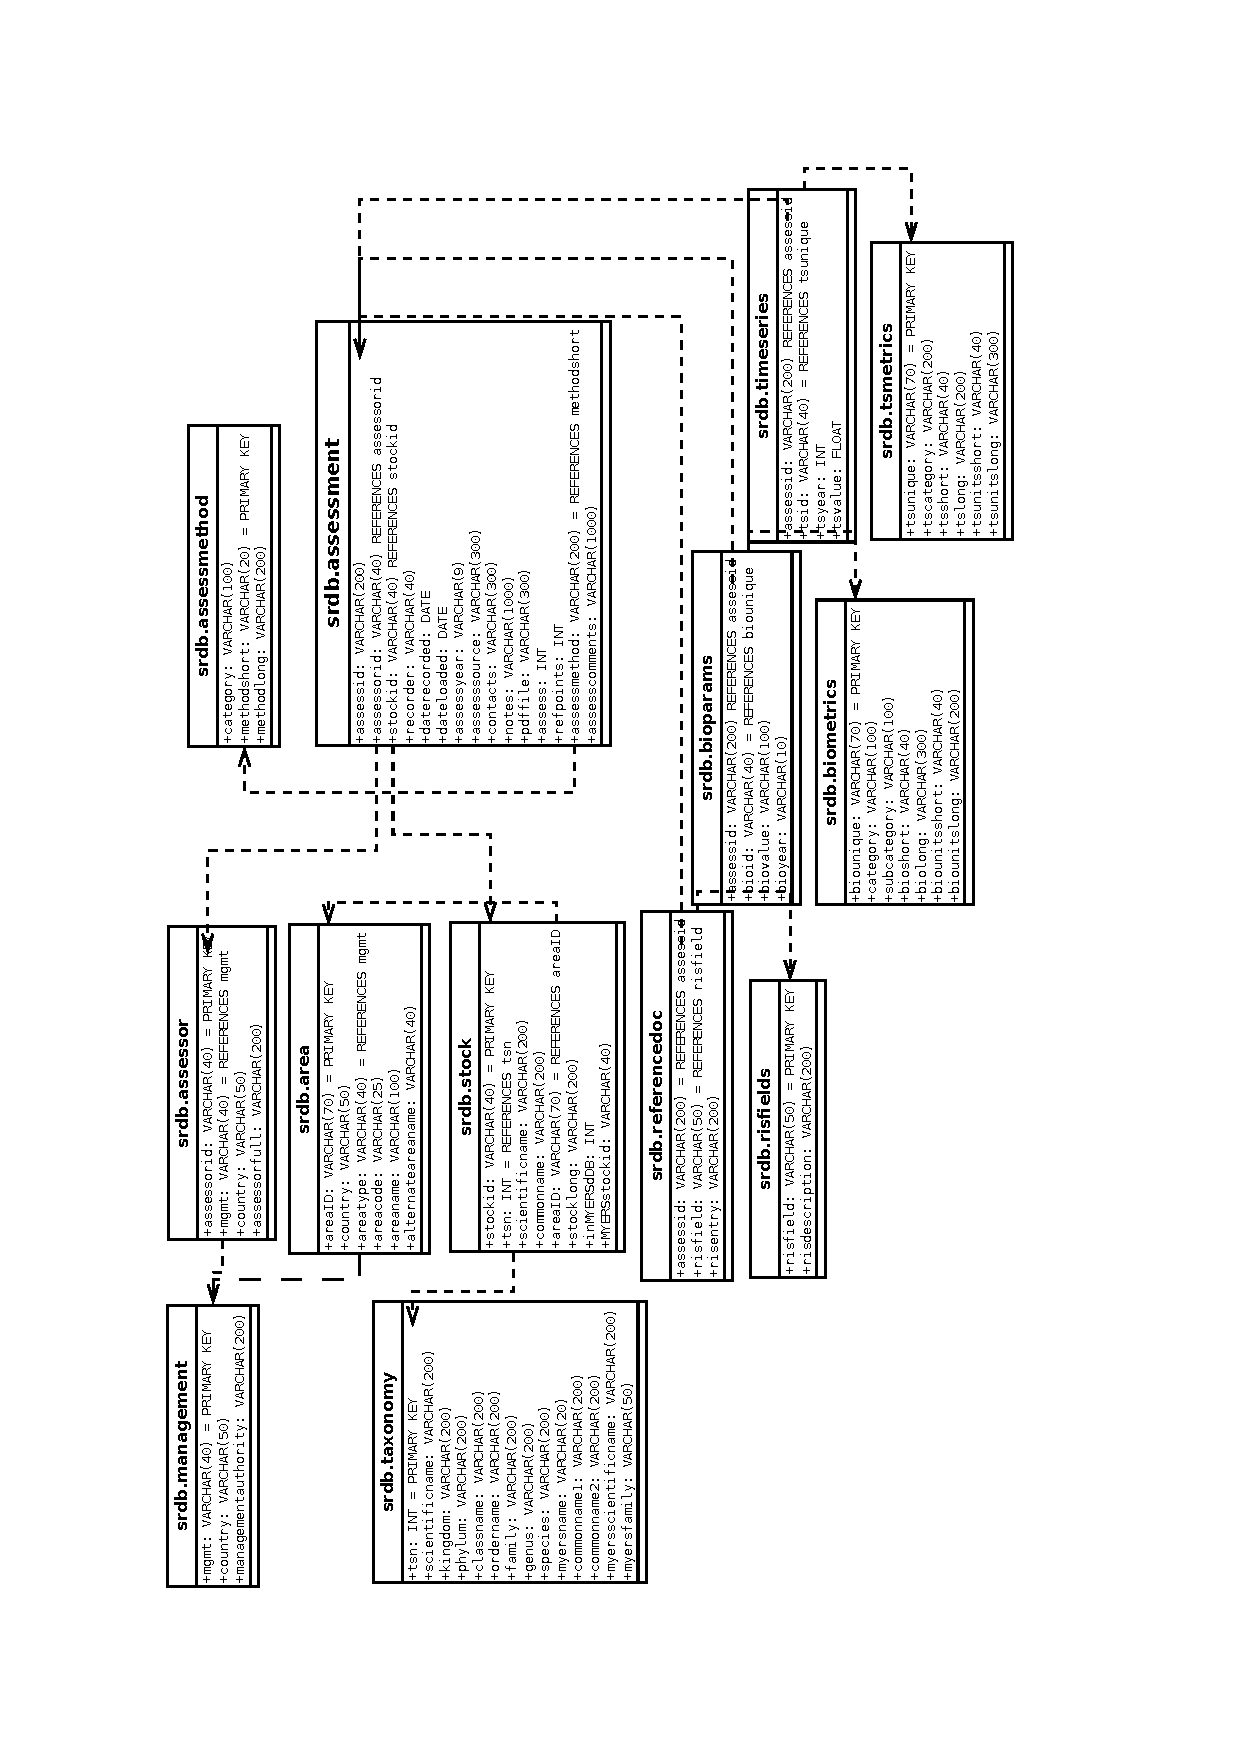
\includegraphics[width=15cm]{/home/srdbadmin/SQLpg/srdb/trunk/doc/srdb-ERD.pdf}%
\lthtmlpictureZ
\lthtmlcheckvsize\clearpage}

{\newpage\clearpage
\lthtmlfigureA{landscape24}%
\begin{landscape}
% latex2html id marker 24

\begin{longtable}{p{1.8cm}p{3.5cm}p{3.5cm}p{3cm}cccp{0.9cm}cp{0.9cm}}
  \bottomrule \\\multicolumn{2}{c}{Continued on next page} \endfoot \endlastfoot
Management & Stock ID & Scientific name & Methodology & Timespan & Current year & B ratio & B ratio from assessment & U ratio & U ratio from assessment  \\\midrule \endhead
AFMA & Bight redfish Southeast Australia & \textit{Centroberyx gerrardi} & Integrated Analysis & 1958-2007 &  &  &  &  &  \\
  AFMA & New Zealand ling Eastern half of Southeast Australia & \textit{Genypterus blacodes} & Integrated Analysis & 1968-2007 & 2007 & 0.59 & yes & 2.20 & no \\
  AFMA & New Zealand ling Western half of Southeast Australia & \textit{Genypterus blacodes} & Integrated Analysis & 1968-2007 &  &  &  &  &  \\
  AFMA & Orange roughy Cascade Plateau & \textit{Hoplostethus atlanticus} & Integrated Analysis & 1987-2006 & 2006 & 1.76 & no & 0.34 & no \\
  AFMA & Orange roughy Southeast Australia & \textit{Hoplostethus atlanticus} & Integrated Analysis & 1978-2007 & 2007 & 0.52 & yes & 0.29 & no \\
  AFMA & Jackass morwong Southeast Australia & \textit{Nemadactylus macropterus} & Integrated Analysis & 1913-2007 & 2007 & 0.31 & yes & 1.80 & no \\
  AFMA & Tiger flathead Southeast Australia & \textit{Neoplatycephalus richardsoni} & Integrated Analysis & 1913-2006 & 2006 & 1.99 & yes & 1.03 & no \\
  AFMA & Northern Australia brown tiger shrimp & \textit{Penaeus esculentus} & Biomass dynamics model & 1970-2006 &  &  &  &  &  \\
  AFMA & Northern Australia grooved Tiger Prawn & \textit{Penaeus esculentus} & Biomass dynamics model & 1970-2006 &  &  &  &  &  \\
  AFMA & Deepwater flathead Southeast Australia & \textit{Platycephalus conatus} & Integrated Analysis & 1978-2007 & 2007 & 1.51 & yes & 0.61 & no \\
  AFMA & Tasmanian giant crab Tasmania & \textit{Pseudocarcinus gigas} & Unknown & 1990-2007 & 2007 & 0.50 & no & 1.71 & no \\
  AFMA & common gemfish Southeast Australia & \textit{Rexea solandri} & Integrated Analysis & 1966-2007 & 2007 & 0.25 & yes & 0.39 & no \\
  AFMA & Blue Warehou Eastern half of Southeast Australia & \textit{Seriolella brama} & Integrated Analysis & 1984-2006 & 2006 & 0.49 & yes & 0.84 & no \\
  AFMA & Blue Warehou Western half of Southeast Australia & \textit{Seriolella brama} & Integrated Analysis & 1984-2006 & 2006 & 0.41 & yes & 2.04 & no \\
  AFMA & Silverfish Southeast Australia & \textit{Seriolella punctata} & Integrated Analysis & 1978-2006 & 2006 & 1.03 & yes & 0.79 & no \\
  AFMA & School whiting Southeast Australia & \textit{Sillago flindersi} & Integrated Analysis & 1945-2007 & 2007 & 0.66 & yes & 0.82 & no \\
  CCAMLR & Antarctic toothfish Ross Sea & \textit{Dissostichus mawsoni} & Integrated Analysis & 1995-2007 & 2007 & 1.76 & no & 0.32 & yes \\
  CFP & Argentine anchoita Northern Argentina & \textit{Engraulis anchoita} & VPA & 1989-2007 & 2007 & 1.37 & yes & 0.17 & yes \\
  CFP & Argentine anchoita Southern Argentina & \textit{Engraulis anchoita} & Biomass dynamics model & 1992-2007 & 2007 & 3.13 & yes & 0.04 & yes \\
  CFP & Patagonian grenadier Southern Argentina & \textit{Macruronus magellanicus} & VPA & 1983-2006 & 2006 & 1.82 & yes & 0.60 & yes \\
  CFP & Argentine hake Northern Argentina & \textit{Merluccius hubbsi} & VPA & 1985-2007 & 2007 & 0.16 & yes & 1.26 & yes \\
  CFP & Argentine hake Southern Argentina & \textit{Merluccius hubbsi} & VPA & 1985-2008 & 2008 & 0.34 & yes & 1.49 & yes \\
  CFP &  Southern blue whiting Southern Argentina & \textit{Micromesistius australis} & VPA & 1985-2007 &  &  &  &  &  \\
  DETMCM & Patagonian toothfish South Africa Subantarctic Prince Edward Islands & \textit{Dissostichus eleginoides} & Biomass dynamics model & 1960-2008 &  &  &  &  &  \\
  DETMCM & Anchovy South Africa & \textit{Engraulis encrasicolus} & Statistical catch at age model & 1984-2006 & 2006 & 0.97 & no & 0.36 & no \\
  DETMCM & Kingklip South Africa & \textit{Genypterus capensis} & Biomass dynamics model & 1932-2008 & 2008 & 1.20 & yes & 0.55 & no \\
  DETMCM & South African abalone South Africa & \textit{Haliotis midae} & Statistical catch at age model & 1951-2008 &  &  &  &  &  \\
  DETMCM & South African west coast rock lobster South Africa Areas 1-2 & \textit{Jasus lalandii} & Statistical catch at age model & 1910-2008 &  &  &  &  &  \\
  DETMCM & South African west coast rock lobster South Africa Areas 3-4 & \textit{Jasus lalandii} & Statistical catch at age model & 1910-2008 &  &  &  &  &  \\
  DETMCM & South African west coast rock lobster South Africa Areas 5-6 & \textit{Jasus lalandii} & Statistical catch at age model & 1910-2008 &  &  &  &  &  \\
  DETMCM & South African west coast rock lobster South Africa Area 7 & \textit{Jasus lalandii} & Statistical catch at age model & 1910-2008 &  &  &  &  &  \\
  DETMCM & South African west coast rock lobster South Africa Area 8 & \textit{Jasus lalandii} & Statistical catch at age model & 1910-2008 &  &  &  &  &  \\
  DETMCM & Shallow-water cape hake South Africa & \textit{Merluccius capensis} & Biomass dynamics model & 1917-2008 & 2008 & 2.30 & yes & 0.40 & no \\
  DETMCM & Deep-water cape hake South Africa & \textit{Merluccius paradoxus} & Biomass dynamics model & 1917-2008 &  &  &  &  &  \\
  DETMCM & Southern spiny lobster South Africa South coast & \textit{Palinurus gilchristi} & Statistical catch at age model & 1973-2008 & 2008 & 0.51 & no & 1.50 & no \\
  DETMCM & Sardine South Africa & \textit{Sardinops sagax} & Statistical catch at age model & 1984-2006 & 2006 & 0.75 & no & 0.55 & no \\
  DETMCM & Cape horse mackerel South Africa South coast & \textit{Trachurus capensis} & Biomass dynamics model & 1950-2007 & 2007 & 1.47 & no & 0.76 & no \\
  DFO & Herring Scotian Shelf and Bay of Fundy & \textit{Clupea harengus} & VPA & 1965-2006 &  &  &  &  &  \\
  DFO & Herring NAFO 4R fall spawners & \textit{Clupea harengus} & VPA & 1971-2003 &  &  &  &  &  \\
  DFO & Herring NAFO 4R spring spawners & \textit{Clupea harengus} & VPA & 1963-2004 &  &  &  &  &  \\
  DFO & Herring NAFO 4T fall spawners & \textit{Clupea harengus} & VPA & 1974-2007 &  &  &  &  &  \\
  DFO & Herring NAFO 4T spring spawners & \textit{Clupea harengus} & VPA & 1974-2007 &  &  &  &  &  \\
  DFO & Pacific herring Central Coast & \textit{Clupea pallasii} & Statistical catch at age model & 1951-2007 & 2007 & 0.30 & no & 0.11 & no \\
  DFO & Pacific herring Prince Rupert District & \textit{Clupea pallasii} & Statistical catch at age model & 1951-2007 & 2007 & 0.16 & no & 0.32 & no \\
  DFO & Pacific herring Queen Charlotte Islands & \textit{Clupea pallasii} & Statistical catch at age model & 1951-2007 & 2007 & 0.20 & no & 0.00 & no \\
  DFO & Pacific herring Straight of Georgia & \textit{Clupea pallasii} & Statistical catch at age model & 1951-2007 & 2007 & 0.91 & no & 0.40 & no \\
  DFO & Pacific herring West Coast of Vancouver Island & \textit{Clupea pallasii} & Statistical catch at age model & 1951-2007 & 2007 & 0.03 & no & 0.00 & no \\
  DFO & Pacific cod Hecate Strait & \textit{Gadus macrocephalus} & Biomass dynamics model & 1956-2005 & 2004 & 0.37 & no & 0.25 & no \\
  DFO & Pacific cod West Coast of Vancouver Island & \textit{Gadus macrocephalus} & Biomass dynamics model & 1956-2002 & 2001 & 0.28 & no & 0.61 & no \\
  DFO & Atlantic cod NAFO 5Zjm & \textit{Gadus morhua} & VPA & 1978-2003 & 2002 & 0.34 & no & 0.45 & no \\
  DFO & Atlantic cod NAFO 2J3KL inshore & \textit{Gadus morhua} & VPA & 1959-2006 & 2005 & 1.60 & no & 0.14 & no \\
  DFO & Atlantic cod NAFO 3Ps & \textit{Gadus morhua} & VPA & 1959-2004 & 2004 & 0.49 & no & 0.41 & no \\
  DFO & Atlantic cod NAFO 3Pn4RS & \textit{Gadus morhua} & VPA & 1964-2007 & 2006 & 0.09 & no & 0.79 & no \\
  DFO & Atlantic cod NAFO 4TVn & \textit{Gadus morhua} & VPA & 1965-2007 & 2006 & 0.17 & no & 0.32 & no \\
  DFO & Rock sole Hecate Strait & \textit{Lepidopsetta bilineata} & Statistical catch at age model & 1945-2001 & 2001 & 1.03 & no & 0.45 & no \\
  DFO & Haddock NAFO-4X5Y & \textit{Melanogrammus aeglefinus} & VPA & 1960-2003 & 2003 & 0.85 & no & 0.33 & no \\
  DFO & Haddock NAFO-5Zejm & \textit{Melanogrammus aeglefinus} & VPA & 1968-2003 & 2002 & 1.00 & no & 0.65 & no \\
  DFO & English sole Hecate Strait & \textit{Parophrys vetulus} & Statistical catch at age model & 1944-2001 & 2001 & 1.23 & no & 0.37 & no \\
  DFO & Pollock NAFO-4VWX5Zc & \textit{Pollachius virens} & VPA & 1974-2007 & 2006 & 0.56 & no & 0.30 & no \\
  IATTC & Yellowfin tuna Eastern Pacific & \textit{Thunnus albacares} & Statistical catch at age model & 1975-2007 &  &  &  &  &  \\
  IATTC & Bigeye tuna Eastern Pacific & \textit{Thunnus obesus} & Integrated Analysis & 1975-2007 &  &  &  &  &  \\
  ICCAT & Skipjack tuna Eastern Atlantic & \textit{Katsuwonus pelamis} & Biomass dynamics model & 1950-2006 & 2006 & 1.71 & no & 0.27 & yes \\
  ICCAT & Skipjack tuna Western Atlantic & \textit{Katsuwonus pelamis} & Biomass dynamics model & 1952-2006 & 2006 & 1.72 & no & 0.32 & yes \\
  ICCAT & Albacore tuna North Atlantic & \textit{Thunnus alalunga} & VPA & 1929-2005 & 2005 & 0.81 & yes & 1.49 & yes \\
  ICCAT & Yellowfin tuna Atlantic & \textit{Thunnus albacares} & VPA & 1970-2006 & 2006 & 1.07 & yes & 0.81 & yes \\
  ICCAT & Bigeye tuna Atlantic & \textit{Thunnus obesus} & Biomass dynamics model & 1950-2005 & 2005 & 0.90 & no & 0.87 & yes \\
  ICCAT & Bluefin tuna Eastern Atlantic & \textit{Thunnus thynnus} & VPA & 1969-2007 & 2007 & 0.34 & yes & 9.38 & yes \\
  ICCAT & Bluefin tuna Western Atlantic & \textit{Thunnus thynnus} & VPA & 1969-2007 & 2007 & 0.57 & yes & 1.33 & yes \\
  ICCAT & Swordfish Mediterranean Sea & \textit{Xiphias gladius} & Biomass dynamics model & 1968-2006 & 2006 & 0.94 & yes & 1.27 & yes \\
  ICCAT & Swordfish North Atlantic & \textit{Xiphias gladius} & Biomass dynamics model & 1978-2007 & 2005 & 0.99 & yes & 0.88 & yes \\
  ICCAT & Swordfish South Atlantic & \textit{Xiphias gladius} & Biomass dynamics model & 1970-2005 & 2005 & 1.54 & yes & 0.49 & yes \\
  ICES & Sandeel North Sea & \textit{Ammodytes marinus} & VPA & 1983-2007 & 2007 & 0.92 & no & 0.24 & no \\
  ICES & Herring ICES 22-24-IIIa & \textit{Clupea harengus} & Statistical catch at age model & 1991-2006 & 2006 & 0.73 & no & 1.02 & no \\
  ICES & Herring Northern Irish Sea & \textit{Clupea harengus} & Statistical catch at age model & 1960-2006 & 2006 & 0.72 & no & 0.34 & no \\
  ICES & Herring North Sea & \textit{Clupea harengus} & Statistical catch at age model & 1960-2007 & 2006 & 0.65 & no & 1.32 & no \\
  ICES & Herring ICES VIa & \textit{Clupea harengus} & Statistical catch at age model & 1957-2006 & 2006 & 0.18 & no & 1.59 & no \\
  ICES & Herring ICES VIa-VIIb-VIIc & \textit{Clupea harengus} & VPA & 1969-2000 & 2000 & 0.50 & no & 1.04 & no \\
  ICES & Herring ICES 25-32 & \textit{Clupea harengus} & VPA & 1973-2006 & 2006 & 0.69 & no & 0.79 & no \\
  ICES & Herring ICES 30 & \textit{Clupea harengus} & VPA & 1972-2007 & 2006 & 1.19 & no & 1.10 & no \\
  ICES & Herring ICES 31 & \textit{Clupea harengus} & VPA & 1979-2006 & 2006 & 0.29 & no & 1.60 & no \\
  ICES & Herring Iceland (Summer spawners) & \textit{Clupea harengus} & VPA & 1983-2007 & 2006 & 1.00 & no & 0.79 & no \\
  ICES & Herring ICES 28 & \textit{Clupea harengus} & VPA & 1976-2007 & 2006 & 1.21 & no & 0.87 & no \\
  ICES & Anchovy ICES VIII & \textit{Engraulis encrasicolus} & Biomass dynamics model & 1986-2007 &  &  &  &  &  \\
  ICES & Atlantic cod coastal Norway & \textit{Gadus morhua} & VPA & 1982-2006 & 2006 & 0.27 & no & 2.17 & no \\
  ICES & Atlantic cod Northeast Arctic & \textit{Gadus morhua} & VPA & 1943-2006 & 2006 & 0.56 & no & 1.42 & no \\
  ICES & Atlantic cod Faroe Plateau & \textit{Gadus morhua} & VPA & 1959-2006 & 2006 & 0.26 & no & 1.52 & no \\
  ICES & Atlantic cod Iceland & \textit{Gadus morhua} & Statistical catch at age model & 1952-2006 & 2006 & 0.46 & no & 1.17 & no \\
  ICES & Atlantic cod Baltic Areas 22 and 24 & \textit{Gadus morhua} & VPA & 1969-2007 & 2006 & 0.36 & no & 1.43 & no \\
  ICES & Atlantic cod Baltic Areas 25-32 & \textit{Gadus morhua} & VPA & 1964-2007 & 2006 & 0.16 & no & 1.46 & no \\
  ICES & Atlantic cod Kattegat & \textit{Gadus morhua} & VPA & 1970-2006 & 2006 & 0.19 & no & 0.31 & no \\
  ICES & Atlantic cod Irish Sea & \textit{Gadus morhua} & VPA & 1968-2006 & 2006 & 0.15 & no & 0.56 & no \\
  ICES & Atlantic cod West of Scotland & \textit{Gadus morhua} & Statistical catch at age model & 1977-2006 & 2006 & 0.12 & no & 0.42 & no \\
  ICES & Atlantic cod North Sea & \textit{Gadus morhua} & VPA & 1962-2007 & 2006 & 0.19 & no & 0.80 & no \\
  ICES & Fourspotted megrim ICES VIIIc-IXa & \textit{Lepidorhombus boscii} & VPA & 1986-2006 & 2006 & 0.70 & no & 1.01 & no \\
  ICES & Megrim ICES VIIIc-IXa & \textit{Lepidorhombus whiffiagonis} & VPA & 1985-2007 & 2006 & 0.43 & no & 1.07 & no \\
  ICES & Capelin Barents Sea & \textit{Mallotus villosus} & Unknown & 1965-2007 & 2006 & 0.17 & no & 0.00 & no \\
  ICES & Capelin Iceland & \textit{Mallotus villosus} & Survey index & 1977-2007 & 2006 & 0.49 & no & 0.85 & no \\
  ICES & Haddock Northeast Arctic & \textit{Melanogrammus aeglefinus} & VPA & 1947-2006 & 2006 & 1.10 & no & 1.06 & no \\
  ICES & Haddock Faroe Plateau & \textit{Melanogrammus aeglefinus} & VPA & 1955-2006 & 2006 & 0.85 & no & 1.07 & no \\
  ICES & Haddock Iceland & \textit{Melanogrammus aeglefinus} & VPA & 1977-2007 & 2007 & 0.98 & no & 1.23 & no \\
  ICES & Haddock Irish Sea & \textit{Melanogrammus aeglefinus} & Survey index & 1972-2006 &  &  &  &  &  \\
  ICES & Haddock West of Scotland & \textit{Melanogrammus aeglefinus} & Statistical catch at age model & 1977-2006 & 2006 & 0.58 & no & 0.73 & no \\
  ICES & Haddock ICES IIIa and North Sea & \textit{Melanogrammus aeglefinus} & VPA & 1963-2006 & 2006 & 0.62 & no & 0.25 & no \\
  ICES & Haddock Rockall Bank & \textit{Melanogrammus aeglefinus} & VPA & 1990-2007 & 2006 & 1.10 & no & 0.52 & no \\
  ICES & Haddock ICES VIIb-k & \textit{Melanogrammus aeglefinus} & VPA & 1993-2006 & 2006 & 1.37 & no & 0.41 & no \\
  ICES & Whiting ICES VIa & \textit{Merlangius merlangus} & Survey index & 1984-2007 &  &  &  &  &  \\
  ICES & Whiting ICES IIIa, VIId and North Sea & \textit{Merlangius merlangus} & VPA & 1979-2006 & 2006 & 0.33 & no & 1.04 & no \\
  ICES & Whiting ICES VIIe-k & \textit{Merlangius merlangus} & VPA & 1982-2007 & 2006 & 0.44 & no & 1.25 & no \\
  ICES & Hake Northeast Atlantic North & \textit{Merluccius merluccius} & VPA & 1977-2007 & 2006 & 1.04 & no & 0.74 & no \\
  ICES & Hake Northeast Atlantic South & \textit{Merluccius merluccius} & VPA & 1982-2007 &  &  &  &  &  \\
  ICES & Whiting Northeast Atlantic & \textit{Micromesistius poutassou} & Integrated Analysis & 1980-2007 & 2006 & 0.67 & no & 1.66 & no \\
  ICES & European Plaice Irish Sea & \textit{Pleuronectes platessa} & Statistical catch at age model & 1962-2006 & 2006 & 1.07 & no & 0.23 & no \\
  ICES & European Plaice ICES VIId & \textit{Pleuronectes platessa} & VPA & 1979-2006 &  &  &  &  &  \\
  ICES & European Plaice ICES IIIa & \textit{Pleuronectes platessa} & VPA & 1976-2006 &  &  &  &  &  \\
  ICES & European Plaice North Sea & \textit{Pleuronectes platessa} & VPA & 1956-2006 &  &  &  &  &  \\
  ICES & European Plaice ICES VIIf-g & \textit{Pleuronectes platessa} & VPA & 1976-2006 & 2006 & 0.65 & no & 0.41 & no \\
  ICES & European Plaice ICES VIIe & \textit{Pleuronectes platessa} & VPA & 1975-2006 & 2006 & 0.51 & no & 1.39 & no \\
  ICES & Pollock Northeast Arctic & \textit{Pollachius virens} & VPA & 1957-2006 & 2006 & 1.70 & no & 0.60 & no \\
  ICES & Pollock Faroe Plateau & \textit{Pollachius virens} & VPA & 1958-2006 & 2006 & 0.99 & no & 1.52 & no \\
  ICES & Pollock ICES IIIa, VI and North Sea & \textit{Pollachius virens} & VPA & 1964-2006 & 2006 & 0.57 & no & 0.97 & no \\
  ICES & Greenland halibut Northeast Arctic & \textit{Reinhardtius hippoglossoides} & VPA & 1959-2007 & 2006 & 0.36 & no & 1.20 & no \\
  ICES & European pilchard ICES VIIIc-IXa & \textit{Sardina pilchardus} & Statistical catch at age model & 1978-2007 &  &  &  &  &  \\
  ICES & Mackerel ICES Northeast Atlantic & \textit{Scomber scombrus} & Statistical catch at age model & 1972-2007 & 2006 & 0.98 & no & 0.73 & no \\
  ICES & Golden Redfish Northeast Arctic & \textit{Sebastes norvegicus} & Statistical catch at age model & 1986-2006 & 2006 & 0.29 & no & 2.65 & no \\
  ICES & common European sole ICES Kattegat and Skagerrak & \textit{Solea vulgaris} & VPA & 1982-2007 & 2006 & 1.25 & no & 0.54 & no \\
  ICES & common European sole Bay of Biscay & \textit{Solea vulgaris} & VPA & 1982-2006 & 2006 & 0.76 & no & 1.00 & no \\
  ICES & common European sole Irish Sea & \textit{Solea vulgaris} & VPA & 1968-2006 & 2006 & 0.36 & no & 1.16 & no \\
  ICES & common European sole North Sea & \textit{Solea vulgaris} & VPA & 1956-2006 &  &  &  &  &  \\
  ICES & common European sole ICES VIId & \textit{Solea vulgaris} & VPA & 1981-2006 &  &  &  &  &  \\
  ICES & common European sole Celtic Sea & \textit{Solea vulgaris} & VPA & 1970-2006 & 2006 & 0.90 & no & 0.95 & no \\
  ICES & common European sole Western English Channel & \textit{Solea vulgaris} & VPA & 1968-2006 & 2006 & 0.51 & no & 1.74 & no \\
  ICES & Sprat North Sea & \textit{Sprattus sprattus} & Statistical catch at age model & 1995-2007 &  &  &  &  &  \\
  ICES & Sprat ICES Baltic Areas 22-32 & \textit{Sprattus sprattus} & VPA & 1973-2007 & 2006 & 1.13 & no & 1.27 & no \\
  ICES & Norway pout North Sea & \textit{Trisopterus esmarkii} & VPA & 1983-2007 & 2006 & 0.90 & no & 0.33 & no \\
  IMARPE & Peruvian anchoveta North-Central Peru & \textit{Engraulis ringens} & VPA & 1963-2004 &  &  &  &  &  \\
  IOTC & Bigeye tuna Indian Ocean & \textit{Thunnus obesus} & Biomass dynamics model & 1957-2006 & 2004 & 1.23 & yes & 0.97 & yes \\
  IPHC & Pacific halibut North Pacific & \textit{Hippoglossus stenolepis} & Statistical catch at age model & 1988-2009 & 2008 & 0.54 & no & 2.01 & no \\
  MFish & Black oreo West end of Chatham Rise & \textit{Allocyttus niger} & Integrated Analysis & 1973-2007 & 2007 & 0.99 & yes & 0.82 & yes \\
  MFish & Australian salmon New Zealand & \textit{Arripis trutta} & Integrated Analysis & 1975-2006 & 2006 & 1.64 & yes & 0.33 & yes \\
  MFish & New Zealand snapper New Zealand Area 8 & \textit{Chrysophrys auratus} & Integrated Analysis & 1931-2005 & 2005 & 0.35 & yes & 2.50 & yes \\
  MFish & New Zealand ling New Zealand Areas LIN 3 and 4 & \textit{Genypterus blacodes} & Integrated Analysis & 1972-2007 & 2007 & 3.07 & yes & 0.09 & yes \\
  MFish & New Zealand ling New Zealand Areas LIN 5 and 6 & \textit{Genypterus blacodes} & Integrated Analysis & 1972-2007 & 2007 & 3.96 & yes & 0.10 & yes \\
  MFish & New Zealand ling New Zealand Area LIN 6b & \textit{Genypterus blacodes} & Integrated Analysis & 1980-2006 & 2006 & 2.19 & yes & 0.11 & yes \\
  MFish & New Zealand ling New Zealand Area LIN 72 & \textit{Genypterus blacodes} & Integrated Analysis & 1972-2007 & 2007 & 2.49 & yes & 0.32 & yes \\
  MFish & New Zealand ling New Zealand Area LIN 7WC - WCSI & \textit{Genypterus blacodes} & Integrated Analysis & 1972-2008 & 2008 & 2.21 & yes & 0.13 & yes \\
  MFish & New Zealand abalone species New Zealand Area PAU 5A & \textit{Haliotis iris} & Integrated Analysis & 1964-2006 & 2006 & 0.72 & no & 2.83 & no \\
  MFish & New Zealand abalone species New Zealand Area PAU 5B & \textit{Haliotis iris} & Integrated Analysis & 1963-2007 & 2007 & 1.02 & no & 0.59 & no \\
  MFish & New Zealand abalone species New Zealand Area PAU 5D & \textit{Haliotis iris} & Integrated Analysis & 1964-2006 & 2006 & 0.44 & no & 2.10 & no \\
  MFish & New Zealand abalone species New Zealand Area PAU 7 & \textit{Haliotis iris} & Integrated Analysis & 1964-2008 & 2008 & 0.87 & no & 0.94 & no \\
  MFish & Orange roughy New Zealand Mid East Coast & \textit{Hoplostethus atlanticus} & Integrated Analysis & 1981-2004 & 2004 & 1.20 & yes & 0.35 & yes \\
  MFish & Red rock lobster New Zealand area CRA1 & \textit{Jasus edwardsii} & Unknown & 1945-2001 & 2001 & 1.14 & no & 0.88 & no \\
  MFish & Red rock lobster New Zealand area CRA2 & \textit{Jasus edwardsii} & Unknown & 1945-2001 & 2001 & 0.53 & no & 2.12 & no \\
  MFish & Red rock lobster New Zealand area CRA3 & \textit{Jasus edwardsii} & Unknown & 1945-2007 &  &  &  &  &  \\
  MFish & Red rock lobster New Zealand area CRA4 & \textit{Jasus edwardsii} & Unknown & 1945-2005 & 2005 & 0.67 & no & 1.33 & no \\
  MFish & Red rock lobster New Zealand area CRA5 & \textit{Jasus edwardsii} & Unknown & 1945-2002 & 2002 & 0.59 & no & 1.68 & no \\
  MFish & Red rock lobster New Zealand area CRA7 & \textit{Jasus edwardsii} & Unknown & 1976-2005 & 2005 & 0.73 & no & 0.43 & no \\
  MFish & Red rock lobster New Zealand area CRA8 & \textit{Jasus edwardsii} & Unknown & 1976-2005 & 2005 & 0.69 & no & 0.49 & no \\
  MFish & Hoki Eastern New Zealand & \textit{Macruronus novaezelandiae} & Integrated Analysis & 1972-2007 & 2007 & 1.11 & no & 0.33 & no \\
  MFish & Hoki Western New Zealand & \textit{Macruronus novaezelandiae} & Integrated Analysis & 1972-2007 & 2007 & 0.51 & no & 0.57 & no \\
  MFish & Southern hake Chatham Rise & \textit{Merluccius australis} & Integrated Analysis & 1975-2006 & 2006 & 1.77 & yes & 0.12 & yes \\
  MFish & Southern hake Sub-Antarctic & \textit{Merluccius australis} & Integrated Analysis & 1975-2007 & 2007 & 2.91 & yes & 0.11 & yes \\
  MFish & Southern blue whiting Campbell Island Rise & \textit{Micromesistius australis} & Integrated Analysis & 1979-2006 & 2006 & 1.15 & yes & 0.92 & yes \\
  MFish & Trevally New Zealand Areas TRE 7 & \textit{Pseudocaranx dentex} & Integrated Analysis & 1944-2005 & 2005 & 1.44 & yes & 0.83 & yes \\
  MFish & Smooth oreo Chatham Rise & \textit{Pseudocyttus maculatus} & Integrated Analysis & 1979-2006 & 2006 & 2.25 & yes & 0.38 & yes \\
  MFish & Smooth oreo West end of Chatham Rise & \textit{Pseudocyttus maculatus} & Integrated Analysis & 1973-2004 & 2004 & 1.25 & yes & 0.53 & yes \\
  MFish & common gemfish New Zealand & \textit{Rexea solandri} & Integrated Analysis & 1952-2007 & 2006 & 1.64 & yes & 0.43 & yes \\
  NAFO & Atlantic cod NAFO 3M & \textit{Gadus morhua} & VPA & 1959-2008 &  &  &  &  &  \\
  NAFO & Atlantic cod NAFO 3NO & \textit{Gadus morhua} & VPA & 1953-2007 & 2006 & 0.02 & no & 0.27 & no \\
  NAFO & American Plaice NAFO-3LNO & \textit{Hippoglossoides platessoides} & VPA & 1955-2007 & 2006 & 0.08 & no & 0.77 & no \\
  NAFO & American Plaice NAFO-3M & \textit{Hippoglossoides platessoides} & VPA & 1960-2007 & 2007 & 0.13 & no & 0.00 & no \\
  NAFO & Yellowtail Flounder NAFO 3LNO & \textit{Limanda ferruginea} & Biomass dynamics model & 1960-2009 & 2007 & 1.62 & no & 0.15 & no \\
  NAFO & Redfish species NAFO 3LN & \textit{Redfish species} & Biomass dynamics model & 1959-2008 & 2008 & 1.88 & yes & 0.04 & yes \\
  NAFO & Redfish species NAFO 3M & \textit{Redfish species} & VPA & 1989-2006 & 2006 & 0.93 & no & 0.15 & no \\
  NAFO & Greenland halibut NAFO 23KLMNO & \textit{Reinhardtius hippoglossoides} & VPA & 1960-2006 & 2006 & 0.39 & no & 1.73 & no \\
  NMFS & Sablefish Eastern Bering Sea / Aleutian Islands / Gulf of Alaska & \textit{Anoplopoma fimbria} & Statistical catch at age model & 1956-2008 & 2008 & 1.05 & yes & 0.66 & yes \\
  NMFS & Sablefish Pacific Coast & \textit{Anoplopoma fimbria} & Integrated Analysis & 1900-2007 & 2007 & 0.84 & no & 0.69 & yes \\
  NMFS & Ocean quahog Atlantic Coast & \textit{Arctica islandica} & Biomass dynamics model & 1978-2008 &  &  &  &  &  \\
  NMFS & Gray triggerfish Gulf of Mexico & \textit{Balistes capriscus} & Biomass dynamics model & 1981-2004 &  &  &  &  &  \\
  NMFS & Gulf menhaden Gulf of Mexico & \textit{Brevoortia patronus} & Statistical catch at age model & 1964-2004 & 2004 & 1.08 & no & 0.48 & no \\
  NMFS & Atlantic menhaden Atlantic & \textit{Brevoortia tyrannus} & Statistical catch at age model & 1940-2005 & 2005 & 0.47 & no & 0.97 & no \\
  NMFS & Blacknose shark Atlantic & \textit{Carcharhinus acronotus} & Biomass dynamics model & 1950-2005 &  &  &  &  &  \\
  NMFS & Finetooth shark Atlantic & \textit{Carcharhinus isodon} & Biomass dynamics model & 1976-2005 &  &  &  &  &  \\
  NMFS & Blacktip shark Atlantic & \textit{Carcharhinus limbatus} & Biomass dynamics model & 1981-2004 &  &  &  &  &  \\
  NMFS & Blacktip shark Gulf of Mexico & \textit{Carcharhinus limbatus} & Biomass dynamics model & 1981-2004 &  &  &  &  &  \\
  NMFS & Sandbar shark Atlantic & \textit{Carcharhinus plumbeus} & Biomass dynamics model & 1975-2004 &  &  &  &  &  \\
  NMFS & Black sea bass Mid-Atlantic Coast & \textit{Centropristis striata} & Statistical catch at age model & 1968-2007 & 2007 & 0.92 & yes & 0.67 & no \\
  NMFS & Snow crab Bering Sea & \textit{Chionoecetes opilio} & Biomass dynamics model & 1979-2008 & 2008 & 0.55 & yes & 1.49 & no \\
  NMFS & Atlantic herring Northwestern Atlantic Coast & \textit{Clupea harengus} & Statistical catch at age model & 1960-2005 &  &  &  &  &  \\
  NMFS & Pacific herring Prince William Sound & \textit{Clupea pallasii} & Statistical catch at age model & 1980-2006 &  &  &  &  &  \\
  NMFS & Pacific herring Sitka & \textit{Clupea pallasii} & Statistical catch at age model & 1978-2007 &  &  &  &  &  \\
  NMFS & Weakfish Atlantic Coast & \textit{Cynoscion regalis} & VPA & 1981-2008 &  &  &  &  &  \\
  NMFS & Petrale sole Northern Pacific Coast & \textit{Eopsetta jordani} & Integrated Analysis & 1910-2005 & 2005 & 1.87 & yes & 1.26 & no \\
  NMFS & Petrale sole Southern Pacific Coast & \textit{Eopsetta jordani} & Integrated Analysis & 1874-2005 & 2005 & 1.13 & yes & 0.61 & no \\
  NMFS & Red grouper Gulf of Mexico & \textit{Epinephelus morio} & Statistical catch at age model & 1986-2005 & 2005 & 1.27 & yes & 0.73 & yes \\
  NMFS & Snowy grouper Southern Atlantic coast & \textit{Epinephelus niveatus} & Statistical catch at age model & 1961-2002 & 2002 & 0.19 & yes & 3.08 & yes \\
  NMFS & Pacific cod Bering Sea and Aleutian Islands & \textit{Gadus macrocephalus} & Integrated Analysis & 1964-2008 & 2008 & 1.00 & yes & 0.93 & no \\
  NMFS & Pacific cod Gulf of Alaska & \textit{Gadus macrocephalus} & Integrated Analysis & 1964-2008 & 2008 & 0.91 & yes & 0.84 & no \\
  NMFS & Atlantic cod Georges Bank & \textit{Gadus morhua} & VPA & 1960-2008 & 2007 & 0.12 & yes & 0.72 & no \\
  NMFS & Atlantic cod Gulf of Maine & \textit{Gadus morhua} & VPA & 1893-2008 & 2007 & 1.46 & no & 2.40 & yes \\
  NMFS & Witch Flounder NAFO-5Y & \textit{Glyptocephalus cynoglossus} & VPA & 1982-2008 & 2007 & 0.30 & yes & 1.45 & yes \\
  NMFS & Rex sole Gulf of Alaska & \textit{Glyptocephalus zachirus} & Statistical catch at age model & 1979-2008 &  &  &  &  &  \\
  NMFS & Kelp greenling Oregon Coast & \textit{Hexagrammos decagrammus} & Integrated Analysis & 1979-2005 &  &  &  &  &  \\
  NMFS & Flathead sole Bering Sea and Aleutian Islands & \textit{Hippoglossoides elassodon} & Statistical catch at age model & 1977-2008 & 2008 & 1.83 & yes & 0.18 & no \\
  NMFS & Flathead sole Gulf of Alaska & \textit{Hippoglossoides elassodon} & Statistical catch at age model & 1978-2008 &  &  &  &  &  \\
  NMFS & American Plaice NAFO-5YZ & \textit{Hippoglossoides platessoides} & VPA & 1960-2008 & 2007 & 0.70 & yes & 0.30 & no \\
  NMFS & Atlantic Halibut NAFO-5YZ & \textit{Hippoglossus hippoglossus} & Unknown & 1800-2007 &  &  &  &  &  \\
  NMFS & American lobster Georges Bank & \textit{Homarus americanus} & Biomass dynamics model & 1981-2007 &  &  &  &  &  \\
  NMFS & American lobster Gulf of Maine & \textit{Homarus americanus} & Biomass dynamics model & 1981-2007 &  &  &  &  &  \\
  NMFS & American lobster Southern New England & \textit{Homarus americanus} & Biomass dynamics model & 1981-2007 &  &  &  &  &  \\
  NMFS & Northern shortfin squid Northwestern Atlantic Coast & \textit{Illex illecebrosus} & Biomass dynamics model & 1967-2005 &  &  &  &  &  \\
  NMFS & Northern rock sole Eastern Bering Sea and Aleutian Islands & \textit{Lepidopsetta polyxystra} & Statistical catch at age model & 1971-2008 & 2007 & 3.02 & yes & 0.21 & yes \\
  NMFS & Yellowfin sole Bering Sea and Aleutian Islands & \textit{Limanda aspera} & Statistical catch at age model & 1959-2008 & 2008 & 1.94 & yes & 0.62 & yes \\
  NMFS & Yellowtail flounder Cape Cod / Gulf of Maine & \textit{Limanda ferruginea} & VPA & 1935-2008 & 2007 & 0.25 & yes & 1.73 & yes \\
  NMFS & Yellowtail flounder Georges Bank & \textit{Limanda ferruginea} & VPA & 1935-2008 & 2007 & 0.22 & yes & 1.14 & yes \\
  NMFS & Yellowtail Flounder Southern New England-Mid Atlantic & \textit{Limanda ferruginea} & VPA & 1935-2008 & 2007 & 0.13 & yes & 1.61 & yes \\
  NMFS & Golden king crab Aleutian Islands Eastern segment & \textit{Lithodes aequispinus} & Statistical catch at length model & 1990-2007 &  &  &  &  &  \\
  NMFS & Golden king crab Aleutian Islands Western segment & \textit{Lithodes aequispinus} & Statistical catch at length model & 1989-2007 &  &  &  &  &  \\
  NMFS & Monkfish Gulf of Maine / Northern Georges Bank & \textit{Lophius americanus} & Unknown & 1964-2006 & 2006 & 1.73 & no & 0.38 & no \\
  NMFS & Monkfish Southern Georges Bank / Mid-Atlantic & \textit{Lophius americanus} & Unknown & 1964-2006 & 2006 & 1.72 & no & 0.30 & no \\
  NMFS & Tilefish Mid-Atlantic Coast & \textit{Lopholatilus chamaeleonticeps} & Biomass dynamics model & 1973-2008 & 2005 & 0.72 & no & 0.61 & no \\
  NMFS & Tilefish Southern Atlantic coast & \textit{Lopholatilus chamaeleonticeps} & Statistical catch at age model & 1961-2002 & 2002 & 0.90 & yes & 1.55 & yes \\
  NMFS & Mutton snapper Southern Atlantic coast and Gulf of Mexico & \textit{Lutjanus analis} & Statistical catch at age model & 1981-2006 &  &  &  &  &  \\
  NMFS & Red snapper Eastern Gulf of Mexico & \textit{Lutjanus campechanus} & Statistical catch at age model & 1872-2003 &  &  &  &  &  \\
  NMFS & Red snapper Southern Atlantic coast & \textit{Lutjanus campechanus} & Statistical catch at age model & 1945-2006 &  &  &  &  &  \\
  NMFS & Red snapper Western Gulf of Mexico & \textit{Lutjanus campechanus} & Statistical catch at age model & 1880-2003 &  &  &  &  &  \\
  NMFS & Haddock NAFO-5Y & \textit{Melanogrammus aeglefinus} & VPA & 1956-2008 & 2007 & 0.99 & yes & 1.21 & no \\
  NMFS & Haddock Georges Bank & \textit{Melanogrammus aeglefinus} & VPA & 1930-2008 &  &  &  &  &  \\
  NMFS & Silver hake Gulf of Maine / Northern Georges Bank & \textit{Merluccius bilinearis} & Survey index & 1955-2005 &  &  &  &  &  \\
  NMFS & Silver hake Southern Georges Bank / Mid-Atlantic & \textit{Merluccius bilinearis} & Survey index & 1955-2005 &  &  &  &  &  \\
  NMFS & Pacific hake Pacific Coast & \textit{Merluccius productus} & Integrated Analysis & 1966-2008 & 2008 & 1.61 & yes & 0.73 & yes \\
  NMFS & Atlantic croaker Mid-Atlantic Coast & \textit{Micropogonias undulatus} & Biomass dynamics model & 1973-2002 & 2002 & 1.42 & yes & 0.27 & yes \\
  NMFS & Dover sole Gulf of Alaska & \textit{Microstomus pacificus} & Statistical catch at age model & 1978-2010 &  &  &  &  &  \\
  NMFS & Dover sole Pacific Coast & \textit{Microstomus pacificus} & Integrated Analysis & 1910-2005 & 2005 & 1.61 & yes & 0.45 & no \\
  NMFS & Striped bass Gulf of Maine / Cape Hatteras & \textit{Morone saxatilis} & Statistical catch at age model & 1982-2006 &  &  &  &  &  \\
  NMFS & Gag Gulf of Mexico & \textit{Mycteroperca microlepis} & Unknown & 1963-2004 & 2004 & 1.00 & yes & 2.44 & yes \\
  NMFS & Gag Southern Atlantic coast & \textit{Mycteroperca microlepis} & Statistical catch at age model & 1962-2005 & 2005 & 0.94 & yes & 1.31 & yes \\
  NMFS & Yellowtail snapper Southern Atlantic Coast and Gulf of Mexico & \textit{Ocyurus chrysurus} & Statistical catch at age model & 1962-2001 & 2001 & 1.14 & yes & 0.61 & yes \\
  NMFS & Lingcod Northern Pacific Coast & \textit{Ophiodon elongatus} & Integrated Analysis & 1956-2005 &  &  &  &  &  \\
  NMFS & Lingcod Southern Pacific Coast & \textit{Ophiodon elongatus} & Integrated Analysis & 1956-2005 &  &  &  &  &  \\
  NMFS & Red porgy Southern Atlantic coast & \textit{Pagrus pagrus} & Statistical catch at age model & 1972-2004 & 2004 & 0.61 & yes & 0.39 & yes \\
  NMFS & Northern shrimp Gulf of Maine & \textit{Pandalus borealis} & Statistical catch at age model & 1960-2009 & 2008 & 1.58 & no & 0.56 & no \\
  NMFS & Summer flounder Mid-Atlantic Coast & \textit{Paralichthys dentatus} & Statistical catch at age model & 1940-2007 &  &  &  &  &  \\
  NMFS & Red king crab Bristol Bay & \textit{Paralithodes camtschaticus} & Statistical catch at length model & 1960-2008 & 2008 & 1.27 & yes & 1.05 & yes \\
  NMFS & Red king crab Norton Sound & \textit{Paralithodes camtschaticus} & Statistical catch at length model & 1976-2008 &  &  &  &  &  \\
  NMFS & English sole Pacific Coast & \textit{Parophrys vetulus} & Integrated Analysis & 1876-2007 & 2007 & 6.42 & yes & 0.14 & no \\
  NMFS & Atlantic butterfish Gulf of Maine / Cape Hatteras & \textit{Peprilus triacanthus} & Unknown & 1965-2005 &  &  &  &  &  \\
  NMFS & Sea scallop Georges Bank & \textit{Placopecten magellanicus} & Statistical catch at length model & 1964-2006 & 2006 & 1.59 & no & 0.78 & no \\
  NMFS & Sea scallop Mid-Atlantic Coast & \textit{Placopecten magellanicus} & Statistical catch at length model & 1964-2006 & 2006 & 1.00 & no & 0.36 & no \\
  NMFS & Starry flounder Northern Pacific Coast & \textit{Platichthys stellatus} & Integrated Analysis & 1970-2005 & 2005 & 1.10 & yes & 0.33 & no \\
  NMFS & Starry flounder Southern Pacific Coast & \textit{Platichthys stellatus} & Integrated Analysis & 1970-2005 & 2005 & 1.55 & yes & 0.12 & no \\
  NMFS & Atka mackerel Bering Sea and Aleutian Islands & \textit{Pleurogrammus monopterygius} & Statistical catch at age model & 1976-2009 & 2009 & 1.55 & yes & 0.55 & no \\
  NMFS & Alaska plaice Bering Sea and Aleutian Islands & \textit{Pleuronectes quadrituberculatus} & Statistical catch at age model & 1972-2008 & 2008 & 2.46 & yes & 0.07 & yes \\
  NMFS & Pollock NAFO-5YZ & \textit{Pollachius virens} & Survey index & 1963-2007 &  &  &  &  &  \\
  NMFS & Bluefish Atlantic Coast & \textit{Pomatomus saltatrix} & Statistical catch at age model & 1981-2007 & 2007 & 0.81 & no & 0.79 & yes \\
  NMFS & Winter Flounder NAFO-5Z & \textit{Pseudopleuronectes americanus} & VPA & 1982-2007 & 2006 & 0.28 & yes & 0.25 & no \\
  NMFS & Winter Flounder NAFO-5Y & \textit{Pseudopleuronectes americanus} & Unknown & 1982-2008 &  &  &  &  &  \\
  NMFS & Winter Flounder Southern New England-Mid Atlantic & \textit{Pseudopleuronectes americanus} & VPA & 1940-2007 & 2007 & 0.09 & yes & 1.10 & no \\
  NMFS & Longnose skate Pacific Coast & \textit{Raja rhina} & Integrated Analysis & 1915-2007 & 2007 & 1.56 & no & 0.40 & no \\
  NMFS & Greenland turbot Bering Sea and Aleutian Islands & \textit{Reinhardtius hippoglossoides} & Statistical catch at age model & 1960-2009 & 2009 & 1.48 & yes & 0.05 & yes \\
  NMFS & Arrowtooth flounder Bering Sea and Aleutian Islands & \textit{Reinhardtius stomias} & Statistical catch at age model & 1970-2008 & 2008 & 2.70 & yes & 0.31 & no \\
  NMFS & Arrowtooth flounder Gulf of Alaska & \textit{Reinhardtius stomias} & Statistical catch at age model & 1958-2010 & 2010 & 3.02 & yes & 0.28 & no \\
  NMFS & Arrowtooth flounder Pacific Coast & \textit{Reinhardtius stomias} & Integrated Analysis & 1916-2007 & 2007 & 3.81 & yes & 0.21 & yes \\
  NMFS & Atlantic sharpnose shark Atlantic & \textit{Rhizoprionodon terraenovae} & Biomass dynamics model & 1950-2005 &  &  &  &  &  \\
  NMFS & Vermilion snapper Gulf of Mexico & \textit{Rhomboplites aurorubens} & Biomass dynamics model & 1981-2004 &  &  &  &  &  \\
  NMFS & Vermilion snapper Southern Atlantic coast & \textit{Rhomboplites aurorubens} & Statistical catch at age model & 1946-2008 & 2007 & 0.86 & yes & 1.27 & yes \\
  NMFS & Pacific sardine North Pacific & \textit{Sardinops sagax} & Statistical catch at age model & 1981-2008 & 2006 & 1.73 & no & 0.37 & no \\
  NMFS & Pacific sardine Pacific Coast & \textit{Sardinops sagax} & Integrated Analysis & 1981-2007 & 2006 & 1.36 & no & 0.41 & no \\
  NMFS & Pacific chub mackerel Pacific Coast & \textit{Scomber japonicus} & Statistical catch at age model & 1929-2008 &  &  &  &  &  \\
  NMFS & King mackerel Gulf of Mexico & \textit{Scomberomorus cavalla} & VPA & 1992-2001 & 2001 & 0.93 & yes & 0.44 & no \\
  NMFS & King mackerel Southern Atlantic Coast & \textit{Scomberomorus cavalla} & VPA & 1981-2001 & 2001 & 1.35 & yes & 0.56 & no \\
  NMFS & Spanish mackerel Southern Atlantic Coast & \textit{Scomberomorus maculatus} & Statistical catch at age model & 1950-2008 & 2007 & 0.38 & yes & 0.91 & yes \\
  NMFS & Atlantic mackerel Gulf of Maine / Cape Hatteras & \textit{Scomber scombrus} & VPA & 1960-2005 &  &  &  &  &  \\
  NMFS & Windowpane flounder - Gulf of Maine / Georges Bank & \textit{Scophthalmus aquosus} & Survey index & 1975-2007 &  &  &  &  &  \\
  NMFS & Windowpane Southern New England-Mid Atlantic & \textit{Scophthalmus aquosus} & Survey index & 1975-2007 &  &  &  &  &  \\
  NMFS & California scorpionfish Southern California & \textit{Scorpaena guttata} & Statistical catch at age model & 1990-2005 &  &  &  &  &  \\
  NMFS & Cabezon Northern California & \textit{Scorpaenichthys marmoratus} & Integrated Analysis & 1916-2005 & 2005 & 1.04 & yes & 0.99 & no \\
  NMFS & Cabezon Southern California & \textit{Scorpaenichthys marmoratus} & Integrated Analysis & 1932-2005 & 2005 & 0.74 & yes & 0.53 & no \\
  NMFS & Rougheye rockfish Bering Sea and Aleutian Islands & \textit{Sebastes aleutianus} & Statistical catch at age model & 1974-2009 &  &  &  &  &  \\
  NMFS & Rougheye rockfish Gulf of Alaska & \textit{Sebastes aleutianus} & Statistical catch at age model & 1974-2007 &  &  &  &  &  \\
  NMFS & Pacific Ocean perch Eastern Bering Sea and Aleutian Islands & \textit{Sebastes alutus} & Statistical catch at age model & 1974-2009 & 2009 & 1.23 & yes & 0.26 & no \\
  NMFS & Pacific ocean perch Gulf of Alaska & \textit{Sebastes alutus} & Statistical catch at age model & 1959-2008 & 2008 & 1.16 & yes & 0.73 & yes \\
  NMFS & Pacific ocean perch Pacific Coast & \textit{Sebastes alutus} & Statistical catch at age model & 1953-2007 & 2007 & 0.69 & yes & 0.00 & yes \\
  NMFS & Shortraker rockfish Bering Sea and Aleutian Islands & \textit{Sebastes borealis} & Statistical catch at age model & 1977-2008 &  &  &  &  &  \\
  NMFS & Gopher rockfish Southern Pacific Coast & \textit{Sebastes carnatus} & Integrated Analysis & 1965-2005 & 2005 & 2.38 & yes & 0.62 & no \\
  NMFS & Darkblotched rockfish Pacific Coast & \textit{Sebastes crameri} & Integrated Analysis & 1928-2007 & 2007 & 0.73 & yes & 0.31 & yes \\
  NMFS & Widow rockfish Pacific Coast & \textit{Sebastes entomelas} & Statistical catch at age model & 1955-2006 & 2006 & 0.91 & no & 0.05 & yes \\
  NMFS & Acadian redfish Gulf of Maine / Georges Bank & \textit{Sebastes fasciatus} & Statistical catch at age model & 1913-2007 &  &  &  &  &  \\
  NMFS & Yellowtail rockfish Northern Pacific Coast & \textit{Sebastes flavidus} & Integrated Analysis & 1967-2005 & 2005 & 1.36 & yes & 0.51 & no \\
  NMFS & Chilipepper Southern Pacific Coast & \textit{Sebastes goodei} & Integrated Analysis & 1892-2007 & 2006 & 1.43 & no & 0.04 & yes \\
  NMFS & Shortbelly rockfish Pacific Coast & \textit{Sebastes jordani} & Integrated Analysis & 1950-2005 &  &  &  &  &  \\
  NMFS & Cowcod Southern California & \textit{Sebastes levis} & Integrated Analysis & 1900-2007 & 2007 & 0.09 & yes & 0.07 & yes \\
  NMFS & Black rockfish Northern Pacific Coast & \textit{Sebastes melanops} & Integrated Analysis & 1914-2006 & 2006 & 1.37 & no & 0.47 & yes \\
  NMFS & Black rockfish Southern Pacific Coast & \textit{Sebastes melanops} & Integrated Analysis & 1915-2007 & 2007 & 2.23 & yes & 0.33 & yes \\
  NMFS & Blackgill rockfish  Pacific Coast & \textit{Sebastes melanostomus} & Integrated Analysis & 1950-2005 & 2005 & 1.31 & yes & 1.20 & no \\
  NMFS & Blue rockfish California & \textit{Sebastes mystinus} & Integrated Analysis & 1916-2007 & 2007 & 0.75 & yes & 1.19 & yes \\
  NMFS & Bocaccio Southern Pacific Coast & \textit{Sebastes paucispinis} & Integrated Analysis & 1951-2006 & 2006 & 0.32 & yes & 0.10 & yes \\
  NMFS & Canary rockfish Pacific Coast & \textit{Sebastes pinniger} & Integrated Analysis & 1916-2007 & 2007 & 0.85 & yes & 0.02 & yes \\
  NMFS & Northern rockfish Bering Sea and Aleutian Islands & \textit{Sebastes polyspinis} & Statistical catch at age model & 1974-2009 & 2009 & 1.41 & yes & 0.13 & no \\
  NMFS & Northern rockfish Gulf of Alaska & \textit{Sebastes polyspinis} & Statistical catch at age model & 1959-2008 & 2008 & 1.50 & yes & 0.66 & yes \\
  NMFS & Yelloweye rockfish Pacific Coast & \textit{Sebastes ruberrimus} & Integrated Analysis & 1923-2006 & 2006 & 0.38 & no & 0.65 & yes \\
  NMFS & Dusky rockfish Gulf of Alaska & \textit{Sebastes variabilis} & Statistical catch at age model & 1973-2008 & 2007 & 1.54 & yes & 0.54 & yes \\
  NMFS & Shortspine thornyhead Pacific Coast & \textit{Sebastolobus alascanus} & Integrated Analysis & 1901-2005 & 2005 & 1.57 & yes & 0.93 & no \\
  NMFS & Longspine thornyhead Pacific Coast & \textit{Sebastolobus altivelis} & Integrated Analysis & 1962-2005 & 2005 & 2.65 & yes & 0.23 & yes \\
  NMFS & Greater amberjack Gulf of Mexico & \textit{Seriola dumerili} & Biomass dynamics model & 1986-2004 & 2004 & 0.46 & no & 1.52 & no \\
  NMFS & Greater amberjack Southern Atlantic coast & \textit{Seriola dumerili} & Statistical catch at age model & 1946-2006 &  &  &  &  &  \\
  NMFS & Bonnethead shark Atlantic & \textit{Sphyrna tiburo} & Biomass dynamics model & 1950-2005 &  &  &  &  &  \\
  NMFS & Atlantic surfclam Mid-Atlantic Coast & \textit{Spisula solidissima} & Biomass dynamics model & 1965-2008 & 1994 & 1.85 & no & 0.18 & yes \\
  NMFS & Spiny dogfish Atlantic Coast & \textit{Squalus acanthias} & Unknown & 1962-2006 & 2005 & 1.61 & no & 0.15 & no \\
  NMFS & Scup Atlantic Coast & \textit{Stenotomus chrysops} & Statistical catch at age model & 1960-2007 &  &  &  &  &  \\
  NMFS & Walleye pollock Aleutian Islands & \textit{Theragra chalcogramma} & Statistical catch at age model & 1976-2008 & 2008 & 0.86 & yes & 0.02 & yes \\
  NMFS & Walleye pollock Eastern Bering Sea & \textit{Theragra chalcogramma} & Statistical catch at age model & 1963-2008 & 2008 & 0.66 & yes & 0.85 & no \\
  NMFS & Walleye pollock Gulf of Alaska & \textit{Theragra chalcogramma} & Statistical catch at age model & 1964-2008 &  &  &  &  &  \\
  NMFS & White hake Georges Bank / Gulf of Maine & \textit{Urophycis tenuis} & Biomass dynamics model & 1963-2007 & 2007 & 0.35 & yes & 0.80 & yes \\
  RFFA & Walleye pollock Northern Sea of Okhotsk & \textit{Theragra chalcogramma} & Biomass dynamics model & 1985-1994 & 1992 & 1.11 & no & 0.63 & yes \\
  RFFA & Walleye pollock Western Bering Sea & \textit{Theragra chalcogramma} & VPA & 1994-2004 & 2004 & 2.16 & no & 0.26 & no \\
  SPRFMO & Chilean jack mackerel Chilean EEZ and offshore & \textit{Trachurus murphyi} & Unknown & 1975-2007 & 2006 & 0.52 & no & 1.20 & no \\
  UNKNOWN & Shortfin mako Nothwest Pacific Ocean & \textit{Isurus oxyrinchus} & VPA & 1990-2003 &  &  &  &  &  \\
  US State & American lobster Rhode Island & \textit{Homarus americanus} & Biomass dynamics model & 1959-2007 & 2006 & 0.53 & no & 0.67 & no \\
  US State & Winter flounder Rhode Island & \textit{Pseudopleuronectes americanus} & Biomass dynamics model & 1959-2007 & 2006 & 0.25 & no & 2.02 & yes \\
  US State & Tautog Rhode Island & \textit{Tautoga onitis} & Biomass dynamics model & 1959-2007 & 2006 & 0.84 & no & 0.59 & no \\
  WCPFC & Skipjack tuna Central Western Pacific & \textit{Katsuwonus pelamis} & Statistical catch at age model & 1972-2006 & 2006 & 4.38 & yes & 0.30 & yes \\
  WCPFC & Albacore tuna South Pacific Ocean & \textit{Thunnus alalunga} & Statistical catch at age model & 1959-2006 & 2006 & 2.46 & yes & 0.90 & yes \\
  WCPFC & Yellowfin tuna Central Western Pacific & \textit{Thunnus albacares} & Statistical catch at age model & 1952-2005 & 2005 & 1.22 & yes & 0.80 & yes \\
  WCPFC & Bigeye tuna Western Pacific Ocean & \textit{Thunnus obesus} & Statistical catch at age model & 1952-2006 & 2006 & 1.06 & yes & 1.38 & yes \\
   \hline
\hline
\caption{Summary of population-dynamics model based assessments in the RAM Legacy database, including the management body (acronyms from Table 1), assessment method, timespan of their longest time series data, estimated ratios of current biomass to the biomass at MSY and current harvest rate to the harvest rate that results in MSY. Estimated ratios were preferentially obtained directly from the assessment document or derived from surplus production models. When both SSBmsy and Bmsy reference points were available, SSB was chosen preferentially.}
\end{longtable}
\end{landscape}%
\lthtmlfigureZ
\lthtmlcheckvsize\clearpage}

{\newpage\clearpage
\lthtmlinlinemathA{tex2html_wrap_inline393}%
$<$%
\lthtmlinlinemathZ
\lthtmlcheckvsize\clearpage}

{\newpage\clearpage
\lthtmlinlinemathA{tex2html_wrap_inline395}%
$>$%
\lthtmlinlinemathZ
\lthtmlcheckvsize\clearpage}


\end{document}
